%!TEX root = hcwsa.tex

\chapter{在亚琛学习和生活}\label{chap:在亚琛学习和生活}

\section{学习、实习和科研}\label{sec:学习、实习和科研}

  \subsection{学期注册}\label{subsec:学期注册}

    学期注册就是指学期费。如RWTHonline的Studienbeitragsstatus所示,学期费包括社区服务费、交通费、RWTH学生会会费等。学校会给每个学生发邮件,只需在缴费deadline前按Studienbeitragsstatus的指引用银行交钱即可,无需动身前往SuperC。

  \subsection{选课和考试报名}\label{subsec:选课和考试报名}

    登录RWTHonline,点击Studienübersicht,选择Semesterplan,就能看到自己每个学期的课程和考试并且报名。也可以直接点击Lehrveranstaltungen直接选 (全校范围的) 课,点击Prüfungsanmeldung注册考试。

    各个专业的培养计划上都有专业主修课/Focus of Study,以及Elective Course分支下的专业选修课/Specialisation Course和辅修课/Subsidiary Course。授课方式有讲义课Vorlesung (VO)、习题课Übung (UE)、讲义+习题课 (VU)、实验/实习课Praktikum (PR)等等,对应的学分从5到15 ECTS不等。

    考试的注册往往在学期的期中开放,并也有一个注册期限,过了这个期限如果再去注册就会比较麻烦。因为选课和注册考试是分开的,所以您可以通过旁听不同的课程来开阔眼界。值得注意的是每门考试仅允许两次挂科,第三次挂科则无法继续就读与该学科有关的专业,所以各位同学要认真对待每一次考试。

    除了本学期和本专业的课程和考试之外,如果学有余力,您可以提前报名自己专业高学期的课程和考试,以及别的专业的课程和考试,选课和计入学分都很自由。对于别的专业的课程的考试,如果它出现在Semesterplan上,则可被当做辅修课来计入学分;如果它不出现在Semesterplan上,则注册考试的时候须跟您本专业的Studienberater联系,让ta在系统上给您开放个考试注册通道,这样您就可以选择该课的考试,若通过则可顺利计入学分。

    RWTH有一个福利是毕业之际可以移除不良成绩——就是那些虽然已通过但会拉低总绩点的专业选修课和辅修课的成绩,只要Elective Course的分已经修满了的话;但是专业主修课的成绩不能移除。这通常是在学位论文答辩以后的一周内前往ZPA办公室办理。届时,具体操作方式请联系您本专业的Studienberater。

  \subsection{自习室}\label{subsec:自习室}

    Fig.10展示了Audimax (中图实线\& 左图) 和C.A.R.L. (中图虚线\&右图) 的相对位置。这两栋楼都承包各类Vorlesung;Audimax通常是举办RWTH的Welcome week的地点。在演讲厅外面就是自习专用桌。

    Fig.11展示了SuperC的周边建筑分布。SuperC前的大路叫Templergraben (左上直线)。SuperC前方地下一层是Sparkassen Forum (左上箭头\&右上)。位于Templergraben左侧的是两个图书馆Bibliothek (左上实线\&左下),右侧的是Semi90 (左上点线\&右下)。图书馆有用于学生团队讨论的研讨室,需在RWTHonline上预订。

    Fig.12展示了如何从Templergraben (左图直线)前往Mogam自习室。

    登录RWTH Aachen的官网可以查询到学校所有的81个自习室,或者网上搜索自习室的名字也可以得到相关的开放时间信息。各个自习室的开放和关门时间都不同,一到考试季自习室的位置便会极为紧张。

    自习室都保证一张桌子的每个位置能使用电源,比较别致的是从天花板吊下来的电源,如Fig.13所示。

  \subsection{学习资源}\label{subsec:学习资源}

    RWTH提供丰富的学习资源,包括但不限于下面所列的内容——

    \begin{itemize}
      \item RWTHmoodle:所有在RWTHonline上报名的课程都能在RWTHmoodle上找到,截图如B.7.2节的Fig.8所示。课上教授用于授课的材料一般都会上传到RWTHmoodle,学生通过该系统提交作业,助教也通过该系统批改作业。此外,教授会通过该系统发布Ankündigung ,学生可在Forum里讨论组队和作业,教授和助教也会及时回答Forum里的问题。Ankündigung和Forum的所有更新都会邮件发送给您的rwth-aachen.de后缀的邮箱。
      \item 学校官方的VPN:可以通过此VPN从外网登录学校的高性能计算集群 (HPC cluster) 以及下载不开放获取的学术文献1。
      \item Studydrive:适用于各个学科同学使用的资源分享网站。在网站或App上可以根据自己的需求加入Kurse和Gruppen。每个人都可以免费下载以及上传学习资料。Studydrive同时也是一个交流的平台,大家可以自由提出或者回答各种课程相关问题。
      \item Maschboard:机械专业的同学还能使用的类似于Studydrive的网站。在注册之后同样可以在搜索栏里查找相关学习内容。
      \item GigaMove:用于管理提交作业的附件。部分课程的作业要求以此方式上传。
    \end{itemize}

    此外还有非官方的学习资源,包括但不限于——

    \begin{itemize}
      \item libgen:用于爬各种pdf或djvu电子书。自然科学的几乎所有领域的已出版的书籍基本上都能从这里免费下载。
      \item sci-hub:是著名的文献下载网站。对RWTH没有订阅的那些学术期刊可用sci-hub下载文献。出于尊重版权的考虑,能通过RWTH的VPN打开的文献都尽量通过该期刊下载 :)
    \end{itemize}

  \subsection{HiWi}\label{subsec:HiWi}

    HiWi 是Hilfswissenschaftler 的缩写。HiWi可以细分为Studentische Hilfskraft和Wissenschaftliche Hilfskraft。Studentische Hilfskraft没有学位要求,Bachelor在读学生也可以申请。Wissenschaftliche Hilfskraft 则是以已经取得Bachelor或者Master学位为前提。工作内容具体视博士生导师的要求而定,比如编程、实验、建模等等。学有余力的同学可以在学校网站寻找适合自己的岗位。 

  \subsection{实习 Praktikum}\label{subsec:实习 Praktikum}

    部分专业如机械、经济工程等等需要在毕业前完成Pflichtpraktikum (义务实习),具体的实习时长和要求需参照各个专业的Richtlinie;

    实习,Praktikum,分为两类:一类是Pflichtpraktikum 代表,另一类是Freiwilliges Praktikum代表自愿实习,另一部分专业没有要求义务实习,但同学们同样也可以根据自身情况找Freiwilliges Praktikum来丰富自己的简历。

    那么如何找到合适的实习岗位呢?

    \begin{itemize}
      \item 一些比较大的网站如Monster,Stepstone,Jobsuma。可以在Vertragsarten里选择Praktikum,再输入关键字搜索。
      \item 大公司的网站。像Audi,Bosch,BMW,Daimler,VW等等的大公司都有自己的岗位网页。需要时时关注网页的最新公开的岗位,保证一有合适的岗位就及时申请。
      \item LinkedIn。全球领先的职场社交平台。
      \item 同学、朋友的推荐。一般来说一个实习岗位全年都会需要实习生,所以问问专业相关的在职实习同学很有可能能得到内推面试的机会。
    \end{itemize}

  \subsection{德语学习}\label{subsec:德语学习}

    虽然部分专业 (如物理学硕士) 的入学并不需要德语成绩,该学科的交流也并不需要德语。但出于融入当地文化的考虑还是建议学习。通过RWTHonline点击Sprachenzentrum了解德语课和分级考试。

  \subsection{项目-、本科-和硕士论文}\label{subsec:项目-、本科-和硕士论文}

    即Projektarbeit,Bachelorarbeit和Masterarbeit。在修到一定的学分之后,可以选择开始写论文。不同专业开始写论文的条件也各不相同。具体条件可以在各个专业对应的Amtliche Bekanntmachung找到。

    Bachelorarbeit (BA)和Masterarbeit (MA)的开始时间以教授在Erfassungsbogen上签名的日期为准。BA的完成时间最短8周,最长10周 (在有合理理由的情况下最多能延长4周)。MA的完成时间最短18周,最长22周 (在有合理理由的情况下最多能延长6周)。为了避免论文超出规定时间的情况,可以在导师的帮助下制作一个大概的规划,根据自身情况先做一些论文的准备工作再去anmelden。

    机械专业的同学还需要在学期中完成一个Projektarbeit (PA)。PA是以2-5人的小组为单位,需在anmelden之后的三个月内完成 (最多可以延长2周)。

    您可在学校网站找到适合自己专业研究方向的论文题目。

\section{交通}\label{sec:交通}

  德国的公共交通以其四通八达、方便快捷、设施人性化著称,公交车内有专门的婴儿车专区,靠边停车车身侧向倾斜方便乘客下车,残疾人上下公交车也有司机帮忙,等等。德国的``严谨'',也体现在了当地的公共交通时刻表上:即使是一趟小小的乡村公交,都有其明确的时刻表。除此之外,德国大学生每学期享有的一大福利就是学期票,可以在学校所在的州范围内免费乘坐绝大多数的公共交通工具。

  虽然如此,德国的公交其实并不很准时,而是经常延误,尤其在大城市和早晚高峰期间,由于堵车、维修、突发事件等原因造成的延误司空见惯,同时所有线路在周末和节假日都会减少车次 (如周日每一小时一班公交车等),若在此期间出行请提前做好功课,以免造成不必要的麻烦。 

  出了中国,出行查公交,最方便的无疑就是 Google Map,当然误差难免。亚琛市内交通信息查询可以通过手机 App (AVV connect、DB Navigator、ASEAG mobil) 或对应网站查询。

  \subsection{学期票等各类票}\label{subsec:学期票等各类票}

    AVV (Aachen Verkehrsverbund GmbH) 亚琛交通联合有限公司,负责亚琛周围片区、包括StädteRegion Aachen, Kreis Düren, Kreis Heinsberg共涉及 35 个城镇的陆上公共交通。其中包含:公共汽车/Bus,(市内)有轨电车/Straßenbahn/Tram,地铁/U-Bahn,城际高速/S-Bahn,州内短途列车/区域快车/Regional Express (RE)/Regionalbahn (RB),德国高铁/Intercity-Express (ICE/IC)等。在注册完大学后会得到AVV提供的学期票/Semesterticket/Semester Ticket可以在北威州境内乘坐所有除ICE/IC以外的陆上公共交通工具1。荷兰和比利时是跟亚琛接壤的国家,也可凭学期票从亚琛前往特定城市;具体可达地点见C.2.6节。

    ASEAG (Aachener Straßenbahn und Energieversorgungs-AG) 则是负责亚琛当地公共交通的、AVV的子公司。学期票出了什么问题,要打交道的主要还是位于亚琛巴士总站的ASEAG Kundencenter,而不是AVV。

    学期票只有和带有照片的证件一起出示才有效。因此,乘车时请记得将您附有照片的学生证或护照或居留卡随身携带。若未带学期票被查到按照逃票处理,若只带学期票没带学生证会被开罚单之后必须要到ASEAG的办公室报道出示学期票就可以少缴纳罚款。

    关于学期票FAQ:

    1. 我是新生,注册时在RWTHonline那里改信息改晚了,导致没收到学期票,该怎么办?

    答:ASEAG是通过邮寄的方式发放学期票的,而收件人收不到的物品会返还给发件人,也就是ASEAG办公室。如果很久没收到学期票而您的朋友们都收到了,则请带上自己的学生证去ASEAG办公室领取。

    2. 学期票丢了/被偷了,怎么补办?

    答:可携带学生证和有效证件去 ASEAG Kundencenter,可在那里挂失和现场补办,缴纳 10 欧罚款。

    3. 学期票丢了/被偷了以后,朋友可以帮忙过去代办一个新的吗?

    答:找人代办不行,因为补办需要核查本人护照信息。

    4. 是不是注销学籍后学期票就会收回去?

    答:如果 8 月份注销学籍,则应该不能退回学期票的钱,这种情况下应该有权利继续使用学期票直至截止有效期。

    刚到亚琛的同学,总会有或长或短没有学期票的日子。在此期间,若需乘坐公共汽车,就需要购买车票。需要频繁坐车,且暂时没有学期票的同学,可视自身情况购买单程票/Einzel-Tickets,日票/24-Stunden-Ticket,周票/WochenKarte 和月票/MonatKarte,相关信息可在AVV网站上查询。

  \subsection{公交}\label{subsec:公交}

    购票方式有:公交车上向司机购票,自动售票机 (Automaten) (常见于较大的公共车站),网上购票,客服中心 (KundenCentern) 购票。

    公交车票必须打票 (Entwerten) 才能生效,打票机在公交车站、地铁站和火车站入口、巴士和有轨电车上都有。查票人员随机出现,如没有有效车票将会被要求出示身份证件,补齐票款,并被处以 60 欧元的罚款。查票人员有穿制服的,也有便衣,不是每辆车上都会碰到查票人员,因此购票全靠乘客自觉,这也是诚信社会的体现。 

    单程票打票生效后有有效时间,且单程票不得用来乘坐反向回程。大多数公交会规定21:00 后须从司机处上车,并出示有效车票。另外,在火车站和 S-Bahn 车站的德铁运营的红色自动售票机上,也可以购买当地的公交车票,通常在主页面的右下角选项中。需要注意的是,德铁售票机出售的无论是单次票还是天票,都已将购买时间作为生效时间,不适合想要提前购票的乘客。

    乘坐公交时,下车前须摁停车铃通知司机。停车铃一般为红色,上有 ”STOP” 或”Tür auf (开门)” 字样,分布于车厢各处,如门、墙或扶手等,如Fig .14所示。在没有其他乘客上下车的情况下,不摁停车铃,司机可能不停站:这种情形常出现于夜间以及节假日。

    车辆运营的时刻表通常区分为周一至周五(Montag bis Freitag)、周六(Samstag)、周日及节假日(Sonntag und Feiertag),其中工作日班次最多,周日及节假日的班次最少,出行请注意安排。

    公交车上白天和中午一般禁止携带自行车上车,其他时间在车上有足够的位置的前提下周一到周五从19点开始,周六从15点开始周日以及其他法定节假日全天允许每辆公交车携带2辆自行车。除了学期票可以携带自行车外,其他车票均要为自行车买票。

  \subsection{列车}\label{subsec:列车}

    亚琛是个山城,并没有地铁/U-Bahn,但从亚琛主火/Aachen Hbf,西火/Westbahnhof,Schanzbahnhof,Rothe-Erde Bahnhof这几个火车站可以乘坐城际高速/S-Bahn,州内短途列车/区域快车/Regional Express (RE)/Regionalbahn (RB),德国高铁/Intercity-Express (ICE/IC) 等。凭学期票可以在北威州境内乘坐所有除ICE/IC以外的陆上公共交通工具。

    使用学期票可以携带自行车乘坐列车,而其他车票如单次车票、日票、月票等是不可以带自行车上公交的,带自行车上车需要另外购买车票。列车的种类以及学期票可以乘坐的火车类型见C.2.1节。

    列车的门都不是自动开关的,而是需要按门上的开关,如Fig.15的左侧车门所示。停站时开关会有绿色指示灯闪烁。在没有他人上下车的情况下,如不按动开关,车门不会打开。 

  \subsection{自行车}\label{subsec:自行车}

    除了公共交通工具,自行车出行也是众多学生经常使用的代步工具。对于刚来到亚琛的同学可以先租赁自行车,在亚琛主火/Aachen Hbf旁边有一家自行车租赁车行Radstation Aachen可以租到普通的或者电动的自行车。

    一手的自行车可以在亚琛的实体店买到,平均价格在200~400欧元之间,除此之外也能在Amason、eBey线上购买。一些价格优惠质量上乘的二手自行车则可在eBay二手交易网站/eBay Kleineranzeiger或是自行车群里可以找到,还有开学季在SuperC前的自行车二手市场。

    在Super C旁边的VELO - Räder die Bewegen不仅可以购买和维修自行车 (虽然价格小贵),而且还提供免费充气泵和免费工具DIY修车。

    童车/Kinderfahrrad (轮胎尺寸通常为24寸) 对于身高不太高的同学是比较友好的,一来骑得上去,二来价格比成人单车便宜得多。

    作为一个以自行车作为年轻人主要出行方式的大学城,亚琛随处可见如该Fig.14窗外所示的停放杆。

    骑自行车要遵守必要的交通规则,包括但不限于:

    \begin{enumerate}
      \item 车前灯以及车后反射警示灯都要装好;
      \item 除非人行道上铺有自行车专用的红色自行车道 (Fig.16),否则不可在人行道上骑车;
      \item 不得在人行道上的、自行车专用的红色自行车道飙车;
      \item 戴安全帽;
      \item 骑车不可用一只手拿着手机看地图 (正确的习惯应该是买个手机架安在手柄上看);
    \end{enumerate}

    虽违反一两条不至引发处罚阈值,但上述若干条极有可能同时出现在一个不良骑车习惯当中,若被警察蜀黎发现就是数罪并罚 :)

  \subsection{出租车}\label{subsec:出租车}

    除了自己开车或是做朋友的车,出租车可能是最方便的用车叫车出行方式,德国的出租车为淡黄色车身,带有 ”TAXI” 顶灯,其中很大一部分为奔驰品牌,宽敞舒适。

    德国的出租车不能在路边扬招,而是有专门的候车点,包括火车站、长途巴士站、飞机场、公交枢纽站、市中心、旅游热门景点等 (Fig.5上镜了不少出租车,拍摄点正是在亚琛主火/Aachen Hbf)。也可以提前电话预订,上门接送。预订电话可以咨询宾馆前台、旅游信息中心或者通过网络查询,以 ”TAXI” 加上城镇名称即可。 亚琛出租预约电话为0241-22222,0241-66666 或 0241-34441。

    出租车的资费包括起步价(不含任何路程或时间)、公里数、等待时间、行李件数、是否使用信用卡等。城镇间略有差异。支付车费时,应额外支付 10\%左右的小费。还要注意,搭乘出租车的所有乘客都要系好安全带,不系安全带不仅会被司机警告,还可能被警察拦下罚款。如果需要儿童安全座椅,可以提前向出租车公司预订。

  \subsection{城际出行}\label{subsec:城际出行}

    亚琛与比利时和荷兰接壤,拥有三国界碑,一面写着一个国家的名字,被称为是德国 “最国际化的城市”。许多亚琛人住在德国,工作在荷兰,购物在比利时。因为这特殊的地理位置,亚琛的跨境交通非常发达。学期票对部分跨境公交和列车同样适用,可以凭票乘坐公交前往比利时的Kelmis以及荷兰的Vaals和Kerkrade,也可凭票乘坐列车前往荷兰的Maastricht和Heerlen。具体可凭票前往的地点须详询AVV官网。

    亚琛离北威州首府 (北威州第二大城市) 杜塞尔多夫/杜塞/Düsseldorf需2小时列车车程,离北威州第一大的城市科隆/Köln仅1.5小时。这两个城市都有大型机场,国际航班较多。

\section{日常消费和饮食}\label{sec:日常消费和饮食}

  \subsection{支付方式}\label{subsec:支付方式}

    跟国内一样,德国较通用的支付方式为现金、刷卡 (刷储蓄卡或信用卡/VISA)、第三方电子支付。

    德国大部分人还是偏好于现金支付的方式 (德国钱包的小袋子就是用来装硬币的),因为他们担心刷卡或是刷二维码而泄露了自己的信息。部分餐馆因为没有刷卡机而只能使用现金支付 (包括一些中餐馆),所以建议在钱包准备些小额度的现金。

    现金支付有德国特色的自动找零机如Fig.17左图的三个数字所示。往1槽放入硬币,往2槽放入纸币,从3槽找回相应的零钱。不少超市和小餐馆都有自动找零机。

    德银的ATM机 (Fig.17右图) 在亚琛的分布相对较少,相比之下遍地都是ATM机的那个银行是Sparkasse。这涉及到的取钱便捷度的问题已在B.1.4节提及过。注意在欧洲ATM取钱是先退卡再取钱的,国内的则相反。

    刷卡则是用熟悉的POS机,如Fig.17左图的矩形所示,使用方式跟国内一样。不少超市和小餐馆都有POS机。POS机既可刷借记卡也可刷贷记卡。

  \subsection{线上商城}\label{subsec:线上商城}

    所谓第三方电子支付是指PayPal、Sorfot、Sepa等,其角色类似于支付宝和微信钱包,其中PayPal是一款欧美最流行的电子支付App。一个不同是,支付宝和微信钱包在支付时都需要输入密码1,而PayPal在绑定银行卡或信用卡后,在支付过程中就不需要输入密码等任何敏感银行信息2。

    在德国,第三方电子支付的使用场合并不如支付宝/微信支付那样广泛。在须线下交易的场合如超市和小餐馆等就不支持PayPal。在需要线上交易的场合,譬如B.6.1节将谈到的通过Mein Vodafone来充值,就是使用PayPal的一个例子:该App可以使用PayPal或VISA卡给您的手机号码充值;亚马逊虽然是线上商城,但并不支持PayPal付款,而是Amazon账号跟借记卡/贷记卡等卡直接绑定,免密支付。

  \subsection{线下商店-德国超市}\label{subsec:线下商店-德国超市}

    在C.2.4节提及到可以在亚马逊/Amazon1或eBey上购买自行车。这两个网站的确是国外比较常用的线上购物网站,线上版的亚超有开元亚超和亚超在线等。以亚马逊为例,部分商品需要运费,而大多数由亚马逊自营店发货的商品则不需运费;其下单流程跟淘宝并没有太大不同,小小的区别在于亚马逊只需绑定借记卡或贷记卡即可无需输入密码而一键扣款,以至于有时候一不小心手滑下错了单。

    较多不同的则是收货。小哥虽然会尽可能地亲手把快递交给您,或者塞到您的信箱 (如果快递比较小的话),但如果送货时您不在家,他是并不会等特别长时间的:他要么把快递交给您的邻居,要么直接送回当地的分发处。前一种情况还比较好,邻居一般都很nice,几乎没听说过私吞快递的情况;后一种情况就比较糟糕,因为他送过一次之后就不再送了,您得亲自到分发处去取,这么一番折腾是蛮痛苦的。

    德国的主要的几个连锁超市有ALDI、LIDL、Netto、REWE、Edeka、Penny、Kaufland。这些超市基本能满足日常食物所需,如蔬菜、肉类、乳产品、各种生鲜以及 (通过少量加工即可的) 主食。开门时间从早上7点到晚上10点左右。可在上网查找在自己家附近的超市的具体地点和开门时间。

    厨具如锅碗盆瓢可在IKEA、TEDI以及一欧店Euroshop买到。TEDI和Euroshop卖的物品比较杂,包括但不限于办公用品、文具、灯泡电池、杂物袋等,但并不出售现成的食物。IKEA以销售家具类商品闻名,但是亚琛并没有IKEA实体店,而是在隔壁荷兰 :) 欲在亚琛购买家具类商品的替代选择是POCO Einrichtungsmarkt。

    日化用品如沐浴露、洗发水、牙膏、牙刷、洗面乳、剃须刀、卸妆水、化妆品、拖把、抹布、洗衣液洗衣粉等都可以在DM以及ROSSMAN找到。

    亚琛虽小,但也是有大型商场的。AQUIS PLAZA是亚琛的购物中心,MediaMarkt销售电子产品,Kauf Galerie 是欧式服装步行街,Listmann和Müller有精品级的文具、化妆品、办公用品、图书、音像制品。

  \subsection{线下商店-中国超市}\label{subsec:线下商店-中国超市}

    生活在异国他乡,你是不是经常怀念家乡的味道呢?打开柜子,你是不是总是想寻找家乡的食材? 亚琛大大小小的亚超总能帮你找到家乡的感觉。从螺蛳粉到自热火锅,从泡面到烤冷面,只有你想不到,没有你买不到。

    中华行/Sino Store这家亚超位于Super C附近,顺着SuperC向下走,在路的拐角处,店面不是特别明显。麻雀虽小,五脏俱全,在这家亚超你几乎能找到一切。做饭必备的调味品,种类繁多的方便食品,新鲜嫩绿的中国蔬菜,琳琅满目的零食小吃等等,一切应有尽有。到了传统节日,老板/老板娘还会上架自己包的各种口味的粽子,很多外国的朋友都慕名前来品尝。更不用说人美心善的老板/老板娘常常会送你点零食,抹去个零头。各位同学如果没来过的话就快来看看吧!

    万家超市在亚琛的Kaufland旁边,种类齐全,店面较大。乐购超级市场在亚琛主火/Aachen Hbf旁边,种类也很齐全。

  \subsection{大学食堂}\label{subsec:大学食堂}

    亚琛大学生服务中心/Studierendenwerk-Aachen范围内设立了九个食堂涵,盖了不同的饮食需求,为在校学生和教职人员提供了最为便捷的餐饮服务。食堂采取自助餐的形式,学生携带学生卡 (Bluecard或者FH Karte) 即可在此消费,选好喜欢的食物后端到柜台结账即可。

    学生卡的充值方式:

    \begin{enumerate}
      \item 在所有食堂都有自动充值机,可以现金充值也可以刷卡充值。
      \item 在部分食堂的服务柜台可以开通自动充值服务,即签署一个直接付款协议 (SEPA-Lastschriftmandat),学校可以直接从协议中绑定的银行卡里扣款,为您的学生卡充值。开通此服务后,当卡内余额不足时,收银员会询问您是否充值以及充值金额多少,然后直接充值。
    \end{enumerate}

    \textbf{无学生卡的消费方式}:

    如果您想带校外的朋友来食堂就餐,则需要申请Studierendegastkarte或者Gastkarte. 

    \begin{enumerate}
      \item 如果您的朋友是德国高校的大学生,可以在任意自动充值机上花2欧申请一张Studierendegastkarte。结账时需要出示大学学生证,即可享受大学生价格。使用完后,卡片工本费和剩余金额可以在Mensa Academica的Infopoint退回。
      \item 如果您的朋友不是德国高校的大学生,则可以在Infopoint或者任意收银处申请一张Gastkarte。用完后,卡片工本费和剩余金额可以在Infopoint、Mensa Vita (Kaffeebar) 、Mensa Bayernallee (Kaffeebar) 或Mensa Jülich退回。Gastkarte不享受大学生价格。
    \end{enumerate}
    
    每日菜单:

    每个食堂每天都会提供不同的菜肴,你可以通过RWTHApp查看这一周的菜式。B.7.2节的Fig.9点击Canteens (德文版为Mensen) 可以查看Studierendenwerk-Aachen管理的所有食堂的一周菜谱。

    \begin{figure}[h]
    \centering
    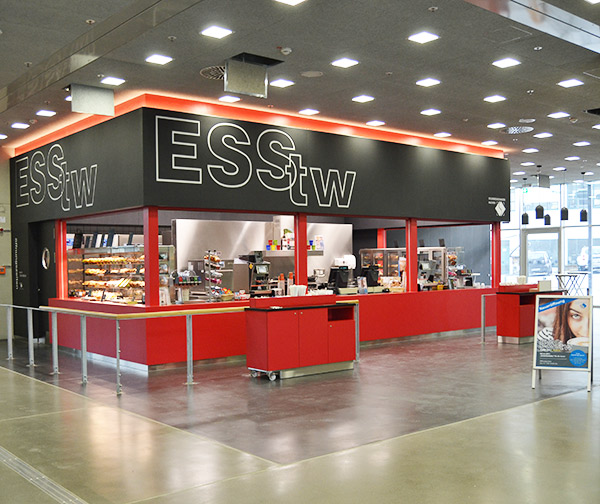
\includegraphics[width=0.19\textwidth]{在亚琛学习和生活/Mensa/ESStW-1.jpg} \ 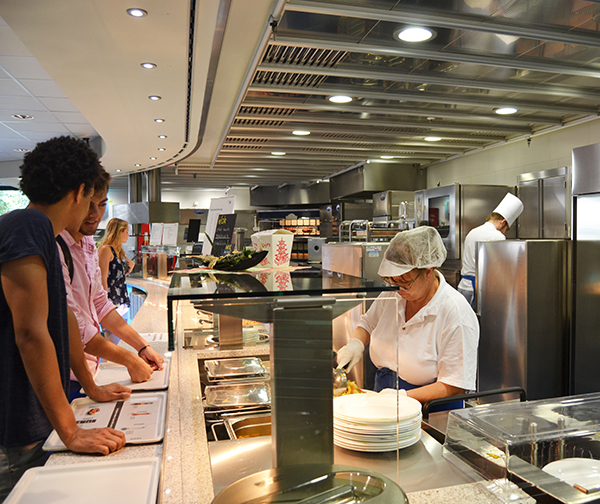
\includegraphics[width=0.19\textwidth]{在亚琛学习和生活/Mensa/Academica 3.jpg} \ 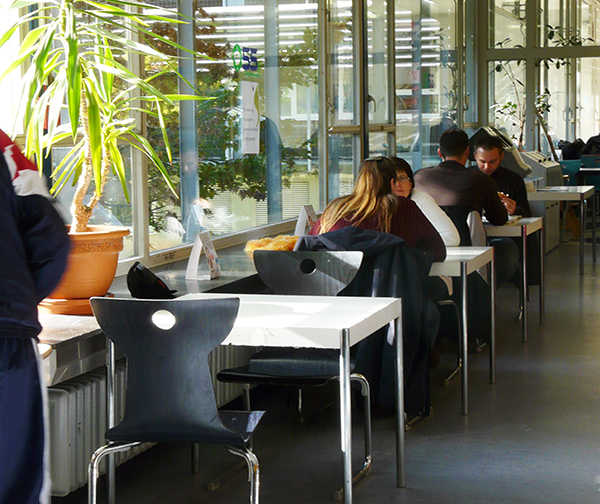
\includegraphics[width=0.19\textwidth]{在亚琛学习和生活/Mensa/MensaAhornstrasse1.jpg} \ 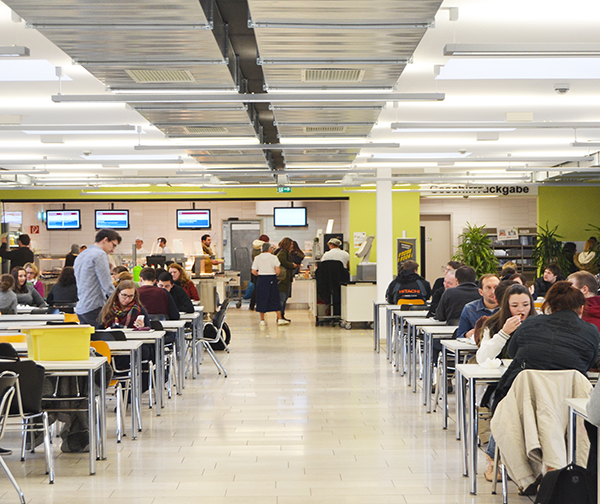
\includegraphics[width=0.19\textwidth]{在亚琛学习和生活/Mensa/Mensa Bayernallee 2.jpg} \ 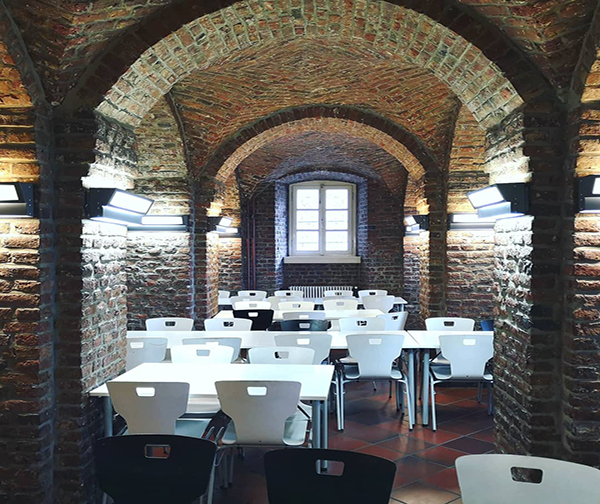
\includegraphics[width=0.19\textwidth]{在亚琛学习和生活/Mensa/Bistro1.jpg}
    \vskip.3\baselineskip
    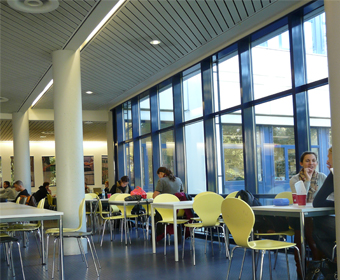
\includegraphics[width=0.19\textwidth]{在亚琛学习和生活/Mensa/mensa Eupener Strasse 2.jpg} \ 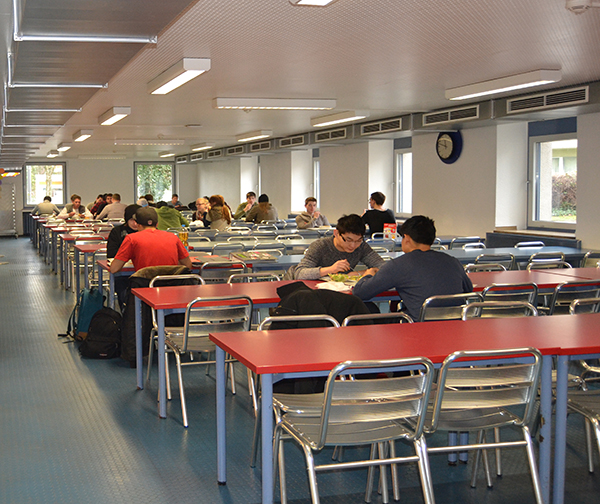
\includegraphics[width=0.19\textwidth]{在亚琛学习和生活/Mensa/Goethestrasse7.jpg} \ 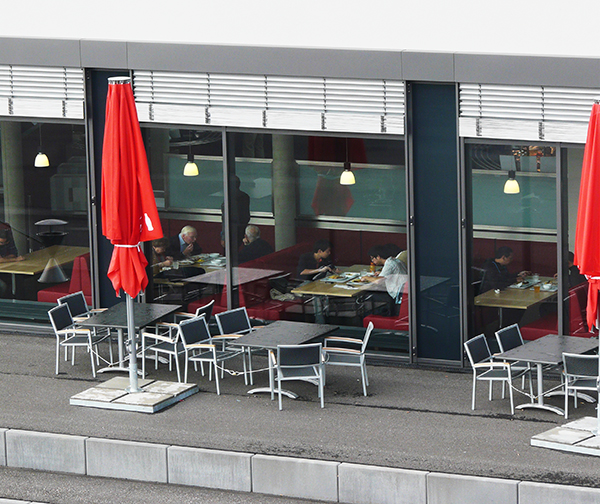
\includegraphics[width=0.19\textwidth]{在亚琛学习和生活/Mensa/mensajuelich6.jpg} \ 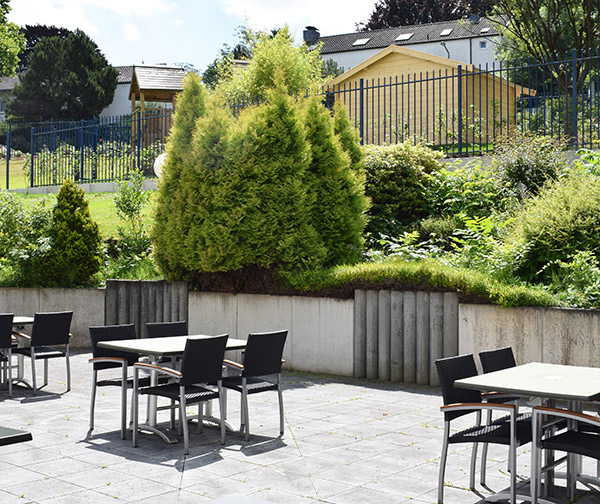
\includegraphics[width=0.19\textwidth]{在亚琛学习和生活/Mensa/Suedpark-1.jpg} \ 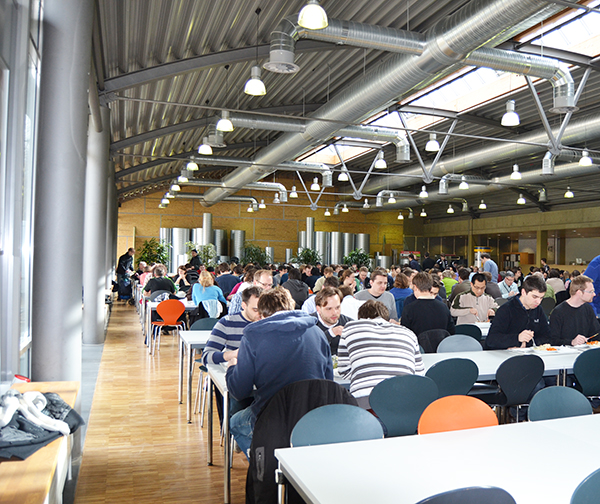
\includegraphics[width=0.19\textwidth]{在亚琛学习和生活/Mensa/MensaVita2.jpg}
    \end{figure}

    Fig.22从左到右从上到下分别为:Cafeteria ESStw, Mensa Academica, Mensa Ahomstraße, Mensa Bayemallee, Mensa Bistro Templergraben, Mensa Eupener Straße, Mensa Goethestraße, Mensa Jülich, Mensa Südpark, Mensa Vita,对应于Fig.9最右图是从上到下的顺序。

  \subsection{中餐馆和亚琛美食街}\label{subsec:中餐馆和亚琛美食街}

    除了大学的食堂,周围还有提供平价盒饭服务的中餐馆;部分餐厅规模较大,适合宴请。在学校周围提供平价中午中餐晚餐的有:

    \begin{itemize}
      \item 大麦/Damai Fresh (Fig.23左图)
      \item 六月/China Restaurant Juno
      \item 食堂/Chic Town
      \item 鑫隆/China-Imbiss Xinlong (Fig.23右图)
    \end{itemize}

    不在教学区但是提供比较精致的中餐馆有:

    \begin{itemize}
      \item 雅/Miyabi Sichuan Kitchen! 
      \item 东方红/Dong Fan Hong – Chinesisches Restaurant
      \item 城市花园/City Garden
      \item 老严/Tan Tasty
      \item 鸭王/Duck-One
    \end{itemize}

    在Bibliothek背后的Ponstraße 是一条亚琛大学美食街道,这里各种美食,汉堡,西餐,中餐,比萨,地中海美食等等,还有各种的Buffet 自助餐等待各位吃货的光临,以下是在Ponstrasse 的几个西式餐厅:

    \begin{itemize}
      \item Kathy’s frietnesse
      \item Vielharmonie 
      \item FOOD BROTHER
      \item Chicken Pont
    \end{itemize}

\section{看病就医和保险}\label{sec:看病就医和保险}

  \subsection{家庭医生和诊所}\label{subsec:家庭医生和诊所}

    家庭医生/Hausartz可以是指全科医生/Allgemeinmediziner或者专科医生/Facharzt,一般在市中经营着自己的诊所/Praxis,或者几个家庭医生联合经营着一家诊所,病人能在诊所里接受大多数疾病的治疗。如果您患有感冒、发烧、拉肚子或眼睛痛等小症状,您最好的选择是去找家庭医生;而形如牙疼、心理问题、甲沟炎等专科病症,您可以去咨询专科医生。通常您不知道自己的病症属于什么类型,家庭医生会是您的首选:他们会给您开推荐信让您到指定的专科诊所就诊。德国的小诊所的检测设备条件大多和国内大型医院相差无几,所以请您放心去诊所就诊,万一得了重症,诊所的医生也会第一时间把您送入大型医院。

    网上搜索Hauszrtz+城市名或Praxis+城市名,即可找到您家附近的诊所,上面会有该诊所联系电话以及网页 (部分诊所没有网站)。这种诊所分散在城市的各个地方,极大地缓解了当地大医院的就诊压力,通常不需预约看诊时段即可前往就诊,现场刷医保卡挂号排队。就诊前建议提前拨打电话咨询相关事项;如需约Termin,可通过电话或在官网上预约。

  \subsection{药店 Apotheke}\label{subsec:药店 Apotheke}

    网上搜索Apotheke即可找到您家附近的医生在看诊后会开立药单,病患可以凭药单到任何药局购买处方药。若投保的是法定医疗保险/公立保险/公保,视医师所开的药单种类而定,处方药由保险公司全额给付或病患负担部分费用。若投保的是私立保险/私保,买药时必须先自费,接着再凭收据向保险公司报销,报销金额依照个人投保额度及保险公司方案有所不同。

    所谓”药单种类”,跟处方签的颜色有关。处方签分为4种,红黄绿蓝。

    红色处方:属于机打处方,一般都是都是法定医保保险,患者不用支付任何费用。

    绿色处方:一般属于非处方,开的是医生建议药品。无论是公保或私保都不报销非处方药,但患者可以选择不购买。

    黄色处方:开具的药品一般都是强力止痛药或者是麻醉剂,医生开得较少且谨慎,医保期限只有7天。

    蓝色处方:用于私立医疗保险报销,保险单位不属于公共医疗保险范围。

    德国的药局夜间和周日不营业,但是各城市每日都有轮流值班的紧急药局,供急症您在夜间或周末取药。可在网上查询当日有哪些紧急药局开门,夜间急诊的医生有时也会主动告知相关信息。

  \subsection{公立医院}\label{subsec:公立医院}

    亚琛唯一的公立医院是校医院/Universitätsklinikum Aachen,她也是全欧洲最大的单体医院建筑之一。一般来说,在德国是不推荐您患有 一些轻状病症去医院就诊,那里大多是针对各种严重伤病的治疗,如恶性肿瘤,严重心脑血管病,需要进行重大器官移植的手术、有可能造成终身残疾的伤病、晚期慢性病、深度昏迷、永久性瘫痪、严重脑损伤、严重帕金森病和严重精神病等,如果您不满足以上条件,推荐您先去诊所,同时也减少资源浪费。

    如果情况紧急不可耽搁 (半夜发烧或者在节假日摔伤),可以直接前往校医院,因为一般诊所晚上和节假日都不营业。也可以呼叫急救医生,电话号码112。大型医院设有24小时的急诊中心(Notfallzentrum),能随时前往,里头有值班的医生问诊。

  \subsection{保险}\label{subsec:保险}

    B.2章提及了公保,其使用方法是看病刷卡挂号,保险公司会直接支付。私保的使用则需先支付挂号费再把账单寄到保险公司审核,保险公司会把报销的钱打回您的账户里。不同的保险有不一样的保障范围。感冒发烧这类小病为所有的保险覆盖。

    在校学生如果年龄超过30岁或者学习时间超过14个学期,公保费用将增至之前的两到三倍,届时可以自由选择留在公保或参加私保。

    除此之外,第三方责任险与法定医疗保险一样属于德国最重要的保险种类之一。虽然是非强制性的,但是为了避免生活中常见的风险,拥有第三方责任险非常必要。比如:弄丢了宿舍楼或家门钥匙;对租房的地面造成了损伤;摔坏了朋友的单反相机等。当索赔人 (第三方) 向您提出理赔要求,保险公司会为您进行调查核实。若参保人有过错需要赔偿第三方时,保险公司会代替您对第三方进行赔偿。若您作为参保人无过错,保险公司会帮助您拒绝并驳回第三方理赔要求。

\section{生活的一切琐碎问题}\label{sec:生活的一切琐碎问题}

  \subsection{垃圾分类和回收}\label{subsec:垃圾分类和回收}

    收件人收不到的物品会返还给发件人

    在德国,垃圾在回收前须进行分类,所属垃圾桶的颜色也不相同。亚琛市官网有垃圾分类专栏。下面简单介绍一下:

    \begin{enumerate}
      \item 有机垃圾 (Bioabfall)-> 有机垃圾桶 (一般为绿色或黑色)
      \item 包装材料 (Verpackung) -> 黄色垃圾袋 (桶)
      \item 废纸 (Papierabfall) -> 蓝色垃圾桶
      \item 旧玻璃 (Altglas) -> 玻璃瓶回收桶 (带押金瓶子pfandflasche除外)
      \item 含有害物质的垃圾 (Schadstoffhaltige Abfälle) -> 固定的回收时间及地点
      \item 其余垃圾 (Restmüll)->灰 (黑) 色垃圾桶
      \item 大型垃圾 (Sperrgut):大型垃圾主要包括床垫,家具,电器等等,关于大型垃圾的回收需向市政府登记预约回收时间。联系电话为0241 /432-18666。
    \end{enumerate}

    注:不同种类的垃圾回收时间往往也不同,具体信息请查阅亚琛市官网有关Abfall内容的页面。

  \subsection{德国邮政}\label{subsec:德国邮政}

    在德国寄信用的比较多的是Deutsche Post,快递则是DHL和Hermes。他们会和分布在德国各地的大大小小的商店合作,因此在亚琛各地都能找到他们的Paketshop,只需网上搜索DHL/Hermes Paketshop就可以找到自己附近的Paketshop。寄信也是同理搜索Deutsche Post Filiale。 除了DHL和Hermes以外还有ups、dpd等快递商,但相较之下门店较少。

    Paketshop可以用来寄快递;同时如果快递寄到您家时您碰巧不在家,快递通常也会被寄到离您较近的Paketshop,通常如果您一个星期内没有去Paketshop领取,则会被退回发件人处;您也可以直接将收货地址设置为某个Paketshop。另外,有些不良快递员可能即使您在家也会显示没有送到,对于这种情况将收货地址设置为Paketshop是一个很好的应对措施。DHL在有些地方还有自己的快递柜,使用方式和国内的快递柜一样。

    DHL和Hermes都有各自对应的APP,可以用于寄快递和追踪包裹,使用起来都非常便捷。

  \subsection{节假日}\label{subsec:节假日}

    德国的法定节假日会因为不同的联邦会有细微的差别,除了法定节假日以外还有学校假日。在学校官网可查看该学期的Lecture-free Days。

  \subsection{法律援助}\label{subsec:法律援助}

    对于生活中遇到需要法律方面专业知识的特别困难的问题,AStA (Allgemeiner Studierendenausschuss)提供律师免费的法律建议。网上或者通过电话预约后,请携带学生证和10欧元的押金。 咨询结束后,会重新拿回押金。需要注意的是法律咨询只能通过AStA的事先安排预约,不能提供无预约咨询。

    AStA提供的法律咨询共分为4种类型:

    Allgemeine Rechtsberatung一般性法律咨询:AStA的律师Drolshagen女士每两周提供一次一般性法律建议,将为您提供所有我们无法提供特殊建议的主题的帮助。 在AStA的开放时间内,必须在社会部/Sozialreferat现场预约。

    Prüfungsrecht考试权:考试法是法律的一个非常特殊的领域,因此AStA每隔14天就会向行政法专业律师提供有关此主题的建议。更多信息也可以通过咨询此电子邮箱pruefungsrecht@asta.rwth-aachen.de获得。

    Mietrecht 租房法:AStA与亚琛租户保护协会合作,每周四下午2点至下午4.30在租户保护协会的所在地提供有关租赁法律的建议。 在此之前,必须在AStA开放时间内在社会部现场预约。

    Ausländer*innenrecht 移民法:Ausländer*innenvertretung (AV)每两周就移民法提供免费咨询。 可从AV的网站上获得更多信息。

  \subsection{心理咨询}\label{subsec:心理咨询}

    学校的学生中央咨询服务处/Zentrale Studienberatung为亚琛工业大学的学生和博士在读的同学在个人压力和危机以及可能影响其学习和博士学习的所有问题时提供心理咨询,例如:工作和学习能力的障碍、学习动机问题、考试和演讲焦虑、其他恐惧、情绪波动、方向或决策困难、联系问题、危机与冲突局势等等。

    欢迎您通过电子邮件(psych.beratung@rwth-aachen.de)与学校的咨询团队联系来预约。如果您还有其他问题和疑虑,或有关于建议的特定要求,请告诉他们,例如,如果您只想从女咨询师或男咨询师那里得到建议,亦或您想要外语建议。目前提供的语言有英语,波兰语,土耳其语或越南语。

  \subsection{突发情况}\label{subsec:突发情况}

    如果您遇到紧急情况请大家熟记一下电话,比如盗窃请在第一时间先联系德国警察,电话:110,另如人身伤害的情况请先联系德国急救电话:112,以及外交部全球领事保护与服务应急呼叫中心电话:+86-10-12308。警方以及急救人员到场后,如仍需帮助可以联系亚琛学联官方微信帐号:RWTHChina,我们会为您提供力所能及的帮助!

\section{休闲娱乐}\label{sec:休闲娱乐}

  \subsection{文娱活动}\label{subsec:文娱活动}

    亚琛常被看成没有太多娱乐活动的大学城市,但仔细寻找,还是有许多可以探索玩乐的地方。亚琛南边有亚琛森林,东南方向有动物园,北边有艾弗尔国家公园/Eifel National Park。

    电影院Cineplex Kinopark Aachen 有上映德语版和英语版的电影。

    喜欢探险冒险的真人CS激光游戏 (Black Laser Tag),组队或是单人的密室逃脱 (Team Escape Aachen)。在鸭王经常举办牌类游戏像是狼人杀,德州扑克,三国杀等。周末坐火车到杜塞还有KTV等娱乐设施。

  \subsection{体育}\label{subsec:体育}

    RwthSport对不同程度的运动爱好者,提供不同等级不同类型的运动课程,比如拳击课有3个等级,不同等级的训练强度不同,如何不清楚自己的等级可以先报名之后联系RwthSportTeam 换课程,在这个网站有78中不同的运动。除了传统篮球,足球,羽毛球,排球。还有像是骑马,高尔夫,击剑,拳击等等很有意思的运动感项目。除此之外rwth 定期给需要户外场地的户外运动举行需要付费的运动度假,像是滑雪,冲浪,帆船。除了Rwth 学校的运动社团,还有些健身房,健身俱乐部,像是Micfit FitX World of Fitness 等等。

  \subsection{学联活动}\label{subsec:学联活动}

    为了丰富亚琛留学生的生活,亚琛学联也会组织各种精彩有趣的活动,比如在德国有宠物就是人生赢家的猫猫摄影大赛,为了与周边其他城市发展革命友谊的联谊会,每年都有的亚琛春晚演出,年年涌现出不同优秀歌手的亚琛好声音。大家可以多多关注学联公众号并参加这些活动。
